\svnid{$Id: ds_guide.tex 1 2015-08-30 15:39:28Z rodriqu_dd $}

\chapter{Piping\label{chap:piping}}

\section{Inleiding}
Dit hoofdstuk beschrijft de procedure om een piping berekening op te zetten en uit te voeren. 

\section{Toevoegen van een piping faalmechanisme}
\label{sec:addpiping}
Om een piping berekening uit te voeren, moet er allereerst een WTI project zitten in het algemeen project. Een WTI project wordt toegevoegd door op het project met de rechter muisknop te klikken, en dan door voor de opties \textit{New} en vervolgens \textit{Item} te kiezen.

\begin{figure} [H]
	\centering
		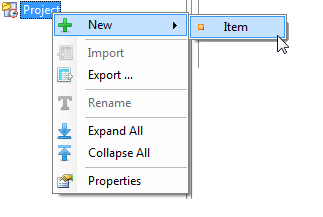
\includegraphics{figures/chapter_piping/addNewProject}
	\caption{Nieuw item toevoegen.}
	\label{fig:fig5.1}
\end{figure}

In de dialoog die dan te zien is, moet er straks gekozen worden voor WTI project.

\begin{figure} [H]
	\centering
		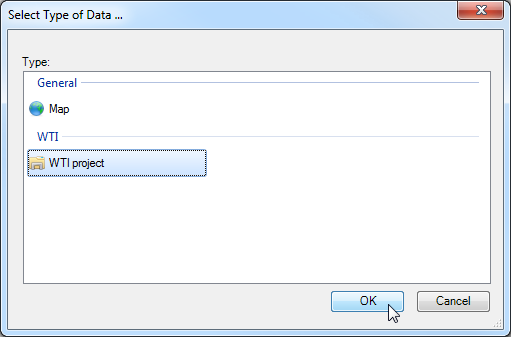
\includegraphics{figures/chapter_piping/selectWTIProject}
	\caption{Nieuw toe te voegen item is WTI project.}
	\label{fig:fig5.2}
\end{figure}

Door gebruik te maken van het contextmenu van het WTI project, kan er uiteindelijk een piping faalmechanisme toegevoegd worden.

\begin{figure} [H]
	\centering
		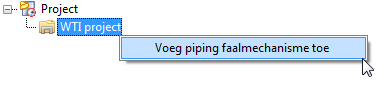
\includegraphics{figures/chapter_piping/addPipingMechanismToProject}
	\caption{Toevoeging van faalmechanisme Piping aan WTI project.}
	\label{fig:fig5.3}
\end{figure}


\section{Piping faalmechanisme berekening uitvoeren}
Als alle invoergegevens voor een piping faalmechanisme berekening klaar zijn, kan deze uitgevoerd worden door op Berekenen te klikken in het contextmenu.

Als de berekening niet uitgevoerd kan worden, dan komt er een bericht terecht in het berichtpanel met verdere informatie over de reden dat het fout is gegaan. Als de berekening wel uitgevoerd is, is het resultaat toegevoegd (of ge\"{u}pdatet) in het projectpanel.





